\documentclass[10pt]{article}

\usepackage{amsfonts}
\usepackage{amsmath}
\usepackage{amssymb}
\usepackage{amsthm}
\usepackage{booktabs}
%\usepackage{mathrsfs}
\usepackage{cite}
%\usepackage{times}
\usepackage{url}
%\usepackage{hyperref}
\usepackage{natbib}
\usepackage{color}
%\hypersetup{
 % bookmarksnumbered = true,
  %bookmarksopen=false,
  %pdfborder=0 0 0,         % make all links invisible, so the pdf looks good when printed
  %pdffitwindow=true,      % window fit to page when opened
  %pdfnewwindow=true, % links in new window
  %colorlinks=true,           % false: boxed links; true: colored links
  %linkcolor=blue,            % color of internal links
  %citecolor=magenta,    % color of links to bibliography
  %filecolor=magenta,     % color of file links
  %urlcolor=cyan              % color of external links
%}
\usepackage{graphicx}
\graphicspath{ {figures/} }

\addtolength{\oddsidemargin}{-.875in}
\addtolength{\evensidemargin}{-.875in}
\addtolength{\textwidth}{1.75in}

\addtolength{\topmargin}{-.875in}
\addtolength{\textheight}{1.75in}

\newcommand{\thornado}{\texttt{thornado}}
\newcommand{\ee}[1]{{\color{blue} #1}}

\begin{document}

\title{Benchmarks of the Non-Relativistic Hydrodynamics Algorithms in \thornado}
%\author{Juliana Pulsinelli\altaffilmark{1} and Eirik Endeve\altaffilmark{2}}

%\altaffiltext{1}{Bearden High School, Knoxville, TN 37919-5449, USA}
%\altaffiltext{2}{Computational and Applied Mathematics Group, Oak Ridge National Laboratory, Oak Ridge, TN 37831-6354, USA; endevee@ornl.gov}

\maketitle

\begin{abstract}
The toolkit for high-order neutrino-radiation hydrodynamics (\thornado) is a code for astrophysical radiation-hydrodynamics based on high-order Runge-Kutta Discontinuous Galerkin (RKDG) methods.  
It currently solves the Euler equations for fluid dynamics and the two-moment ($M_{1}$) approximation of the radiative transfer equation, both in the non-relativistic limits. 
In this document, we benchmark the algorithms for solving the non-relativistic Euler equations.  
Results from an extensive set of one-dimensional Riemann problems are compared to exact solutions in cases where they exist. We also show results for th interacting blast wave problem of Colella and Woodward and the shock entropy wave problem of Shu and Oster. 
\end{abstract}

\tableofcontents

\section{Introduction}

Astrophysical fluid dynamics models the movement of fluids in space. It yields very different solutions from terrestrial fluid dynamics, as the effect of gravity is reduced or removed. 
Fluid dynamics play a major role in the formation of stars and neutron stars, as well as the movement of galaxies and numerous other astrophysical topics.  

\section{Equations and Numerical Method}

In this project, numerical algorithms for solving the Euler equations of fluid dynamics are tested against an extensive suite of standard problems taken from the literature.  
In the following subsections we briefly describe the equations and the numerical methods used.  

\subsection{Euler Equations of Gas Dynamics}

The Euler equations for fluid dynamics \citep[see, e.g.,][for details]{Leveque2002} consists of the mass conservation equation
\begin{equation}
  \frac{\partial \rho}{\partial t}  
  + \frac{\partial}{\partial x} \Big(\rho u\Big) = 0,
  \label{eq:massConservation}
\end{equation}
the momentum conservation equation
\begin{equation}
  \frac{\partial}{\partial t} \Big(\rho u\Big)
  + \frac{\partial}{\partial x} \Big(\rho u^2 + p\Big) = 0,
  \label{eq:momentumConservation}
\end{equation}
and the energy conservation equation
\begin{equation}
  \frac{\partial E}{\partial t}
  + \frac{\partial}{\partial x} \Big((E + p) u\Big) = 0.  
  \label{eq:energyConservation}
\end{equation}
where $\rho$ represents mass density, $u$ the fluid velocity, $p$ the fluid pressure, and $E=e+\frac{1}{2}\rho u^2$ the total energy (internal plus kinetic).  
Equation~\eqref{eq:massConservation} expresses conservation of mass, Equation~\eqref{eq:momentumConservation} expresses conservation of momentum, and equation \eqref{eq:energyConservation} expresses conservation of energy.
The equation of state
\begin{equation}
  p = (\gamma - 1)
  \Big(E - \frac{1}{2} \rho u^2 \Big)
  \label{eq:eos}
\end{equation}
closes the system of equations, and links the pressure to the quantities evolved by Equations \eqref{eq:massConservation}-\eqref{eq:energyConservation}. 
The ratio of specific heats, $\gamma$, is taken to be a constant.  

By defining the vector of conserved variables $\boldsymbol{U}=(\rho,\rho u,E)^{T}$ and the vector of fluxes $\boldsymbol{F}(\boldsymbol{U})=(\rho u,\rho u^{2}+p,(E+p)u)^{T}$ we write the Euler equations as system of conservation laws
\begin{equation}
  \partial_{t}\boldsymbol{U}
  +\partial_{x}\boldsymbol{F}(\boldsymbol{U})
  =0.
\end{equation}

\subsection{Runge-Kutta Discontinuous Galerkin Methods}

In the Runge-Kutta Discontinuous Galerkin \citep[RKDG; cf.][]{cockburnShu_2001} method the solution to the Euler equations is approximated by a local polynomial expansion of the form
\begin{equation}
  \boldsymbol{U}(x,t)
  \approx\boldsymbol{U}_{h}(x,t)=\sum_{j=0}^{k}\boldsymbol{C}_{j}(t)\,\phi_{j}(x),
\end{equation}
where $\{\phi_{j}(x)\}_{j=0}^{k}$ are polynomials of degree at most $k$ and $\boldsymbol{C}_{j}$ are expansion the coefficients to be solved for.  
In \thornado, $\phi_{j}(x)$ are given by Lagrange polynomials.  

The computational domain $D=\{x:x\in[x_{\mbox{\tiny L}},x_{\mbox{\tiny R}}]\}$ is subdivided into $N$ elements $I_{i}=\{x:x\in(x_{i-1/2},x_{i+1/2})\}$ for $i=1,\ldots,N$.  
The width of element $I_{i}$ is then $\Delta x_{i}=x_{i+1/2}-x_{i-1/2}$.  
The semi-discrete DG method is then to find $\boldsymbol{U}_{h}$ such that
\begin{equation}
  \partial_{t}\int_{I_{i}}\boldsymbol{U}_{h}\,\phi_{j}\,dx
  +\big(\widehat{\boldsymbol{F}}\,\phi_{j}|_{i+1/2}-\widehat{\boldsymbol{F}}\,\phi_{j}|_{i-1/2}\big)
  -\int_{I_{i}}\boldsymbol{F}(\boldsymbol{U}_{h})\,\partial_{x}\phi_{j}\,dx=0
  \label{eq:semidiscreteDG}
\end{equation}
for all $\phi_{j}$ and all $I_{i}\in D$.  
In Equation~\eqref{eq:semidiscreteDG}, $\widehat{\boldsymbol{F}}_{i\pm1/2}$ is a numerical flux approximating the flux across the interfaces connecting neighboring elements.  
In \thornado, we have implemented the Local Lax-Friedrichs (LLF), the Harten-Lax-van Leer (HLL), and the HLLC Riemann solvers, but in the numerical experiments presented here, we only use the HLLC solver.  
To complete the spatial discretization, we use Gaussian quadratures to evaluate the integrals in Eq.~\eqref{eq:semidiscreteDG}.  

We apply the method of lines approach to temporal discretization.  
With the spatial discretization specified, the DG problem in Eq.~\eqref{eq:semidiscreteDG} can be viewed as a system of ordinary differential equations (ODEs) for the expansion coefficients $\boldsymbol{C}=\{\boldsymbol{C}_{j}\}_{j=0}^{k}$, i.e.,
\begin{equation}
  d_{t}\boldsymbol{C}
  =\boldsymbol{L}(\boldsymbol{C}),
\end{equation}
which can be discretized in time.  
To this end, we apply the strong stability-preserving Runge-Kutta (SSP-RK) methods of order 1 to 3 \citep{gottlieb_etal_2001}.  
The 1st order method (SSP-RK1) is simply the forward Euler method, while the 2nd and 3rd order methods (SSP-RK2 and SSP-RK3, respectively) can be expressed as convex combinations of forward Euler steps.  
A general $m$-stage Runge-Kutta method is given by
\begin{align}
  \boldsymbol{C}^{(0)}
  &=\boldsymbol{C}^{n} \\
  \boldsymbol{C}^{(i)}
  &=\sum_{l=1}^{i-1}\alpha_{il}\,\big(\,\boldsymbol{C}^{(l)}+\beta_{il}\,\Delta t\,\boldsymbol{L}(\boldsymbol{C}^{(l)})\,\big)
  \quad i=1,\ldots,m \\
  \boldsymbol{C}^{n+1}
  &=\boldsymbol{C}^{(m)},
\end{align}
where $\alpha_{il},\beta_{il}\ge0$ are given by Butcher tables. During time-integration, we apply limiters to the polynomial representation after each stage as a post-processing step.  
We use the TVB limiter of \citet{} to prevent oscillations near discontinuities and the positivity limiter of \citet{ZhangShu2010} to ensure that the density and pressure remain positive.  


In the numerical experiments presented below, we will vary the spatial and temporal order of the method.  
The 1st order method (DG(0)+RK1) uses polynomials of degree $0$ in each element and the forward Euler time integration method, the second-order method (DG(1)+RK2) uses polynomials of degree $1$ combined SSP-RK2 time integration, while the 3rd order method (DG(2)+RK3) uses polynomials of degree $2$ combined SSP-RK3 time integration.  

\section{Numerical Experiments}

The code was tested against a series of one-dimensional Riemann problems. The Riemann problem models a fluid in an area of one-dimensional space. The initial data features one jump discontinuity, and is constant on either side of this discontinuity. The computational domain is divided into space and time cells. The conditions of each cell are advanced forward for all space cells, one time step at a time, according to the Euler equations for fluid dynamics. \citep{Leveque2002}

%models an area with two fluids, each of which has different characteristics, which are separated from one another by a barrier. When the barrier is removed, the Riemann problem solver code models how the fluids mix, determining how different properties of the fluid change at various spatial locations over time. The fields are evolved forward over time based on the Euler equations.

Several tests were used to assess the accuracy of the RKDG method implemented in thornado \citep{LiskaWendroff2003}. 
\begin{table}[h!]
\begin{center}
\begin{tabular}{ |c|c c c|c c c|c c| }
 \hline
 Test & $\rho_L$ & $u_L$ & $p_L$ & $\rho_R$ & $u_R$ & $p_R$ & $x_0$ & $T$ \\
 \hline
 1 & 1 & 0 & 1 & 0.125 & 0 & 0.1 & 0.5 & 0.2 \\
 2 & 1 & 0.75 & 1 & 0.125 & 0 & 0.1 & 0.3 & 0.2 \\
 3 & 1 & -2 & 0.4 & 1 & 2 & 0.4 & 0.5 & 0.15 \\
 4 & 1 & 1 & $10^{-6}$ & 1 & -1 & $10^{-6}$ & 0.5 & 1 \\
 5 & 1 & -19.59745 & 1000 & 1 & -19.59745 & 0.01 & 0.8 & 0.012 \\
 6 & 5.99924 & 19.5975 & 460.894 & 5.99242 & -6.19633 & 46.095 & 0.4 & 0.035 \\
 7 & 1.4 & 0 & 1 & 1 & 0 & 1 & 0.5 & 2 \\
 8 & 1.4 & 0.1 & 1 & 1 & 0.1 & 1 & 0.5 & 2 \\
 9 & 0.1261192 & 8.9047029 & 782.92899 & 6.591493 & 2.2654207 & 3.1544874 & 0.5 & 0.0039 \\
10 & 5.6698 & 9.0299 & 100 & 1.0 & 0.0 & 1.0 & 0 & 1 \\
11 & 5.6698 & -1.4701 & 100 & 1.0 & -10.5 & 1.0 & 0 & 1 \\
 \hline
\end{tabular}
  \caption{Initial parameters for most of the tests described in this paper, from \citep{LiskaWendroff2003}~and \citep{Leveque2002}. The table shows initial density ($\rho$), velocity ($u$), and pressure ($p$) on both sides of a discontinuity located at $x_0$. These initial conditions are then advanced to time $T$.}
  \label{tab:testtable}
\end{center}
\end{table}
Table 1 dispplays the initial data for the Riemann problems. ($\rho_L$, $u_L$ , $p_L$) denote the mass density, velocity, and pressure to the left of the interface at $x=x_0$;($\rho_R$, $u_R$,  $p_R$) refer to these same quantities to the right of the interface. The problem is advanced to time T.
The computational domain $D$ is defined with $x_{\mbox{\tiny L}}=0.0$ and $x_{\mbox{\tiny R}}=1.0$ in tests 1--8, $x_{\mbox{\tiny L}}=0.1$ and $x_{\mbox{\tiny R}}=0.6$ in test 9 \citep{LiskaWendroff2003}, $x_{\mbox{\tiny L}}=-5$ and $x_{\mbox{\tiny R}}=15$ in test 10, and $x_{\mbox{\tiny L}}=-15$ and $x_{\mbox{\tiny R}}=5$ in test 11 \citep{Leveque2002}. 
%\ee{Provide more detailed description of the Riemann problems and refer to Table~\ref{tab:testtable}}

Test 12 is the Woodward-Collela blast wave problem, computed on 0.0 to 1.0, with discontinuities at 0.1 and 0.9. At all positions, initial density is 1 and initial velocity is 0. Initial pressure is 1000 on the left, 0.01 in the center, and 100 on the right, and the test is advanced to 0.038 seconds. \citep{LiskaWendroff2003}. Test 13 shows Shock Entropy Wave interactions, advanced to 1.8 seconds.
%\clearpage
\subsection{Linear Waves Tests}

\begin{figure}
  \begin{center}
	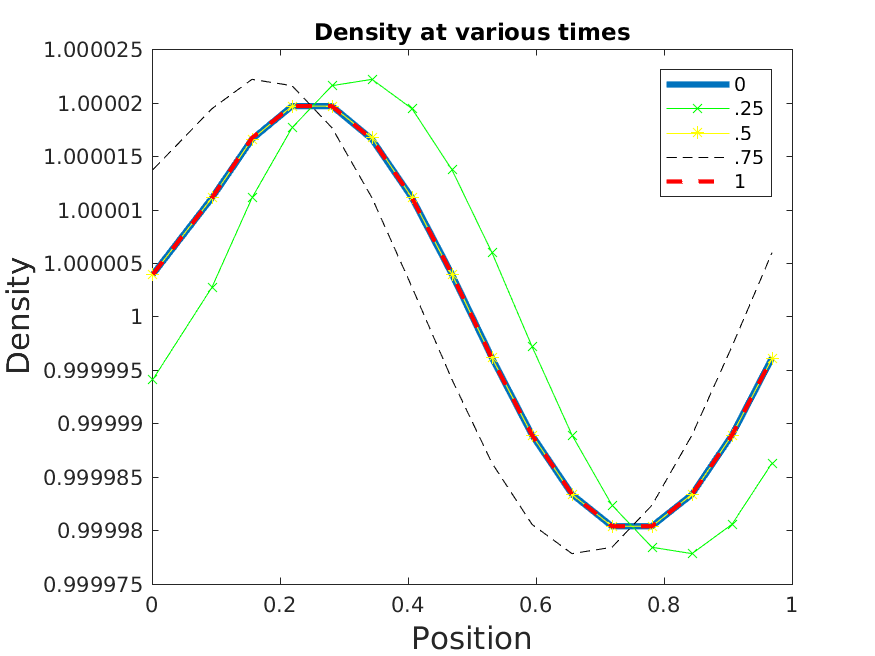
\includegraphics[width=.975\textwidth]{lw1den.png}
	\begin{tabular}{cc}
	  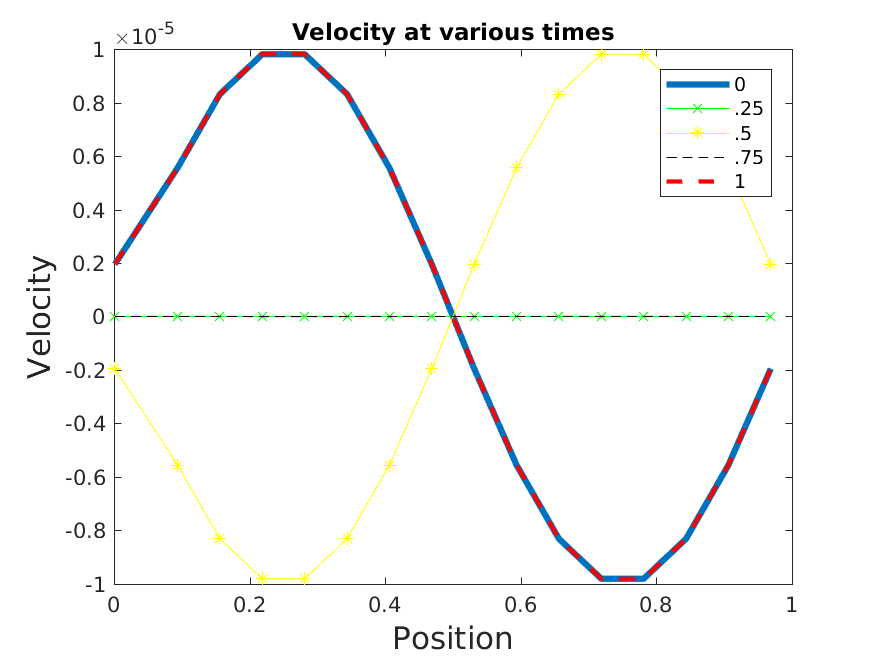
\includegraphics[width=.475\textwidth]{lw1vel.png} &
	  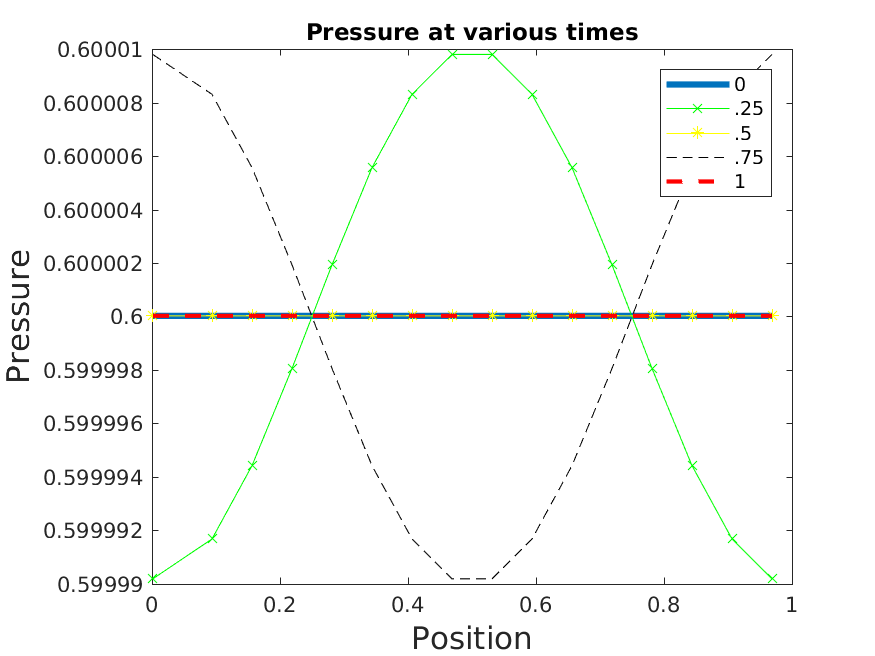
\includegraphics[width=.475\textwidth]{lw1prs.png}
	\end{tabular}
  \end{center}
  \caption{Results from linear waves tests, showing density (top), velocity (bottom left) and pressure (bottom right) computed at various times after a disturbance.}
  \label{fig:lw1}
\end{figure}
\clearpage

\begin{figure}
  \begin{center}
	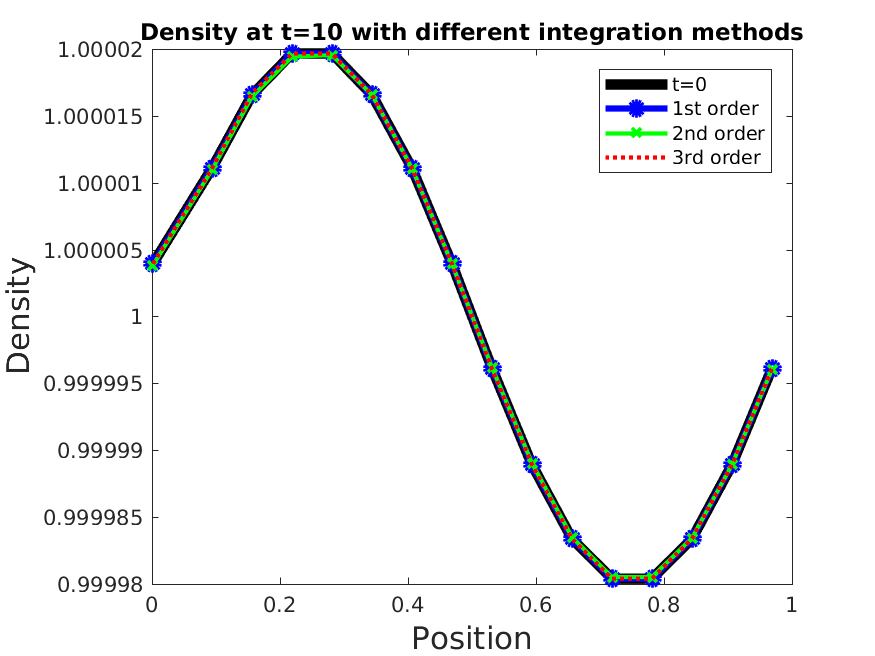
\includegraphics[width=.975\textwidth]{lw2den.png}
	\begin{tabular}{cc}
	  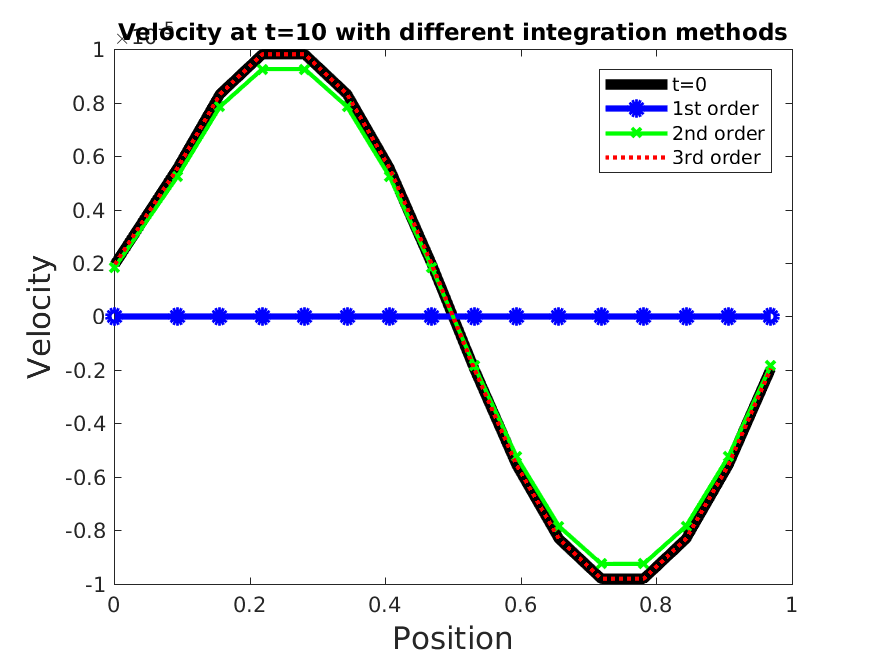
\includegraphics[width=.475\textwidth]{lw2vel.png} &
	  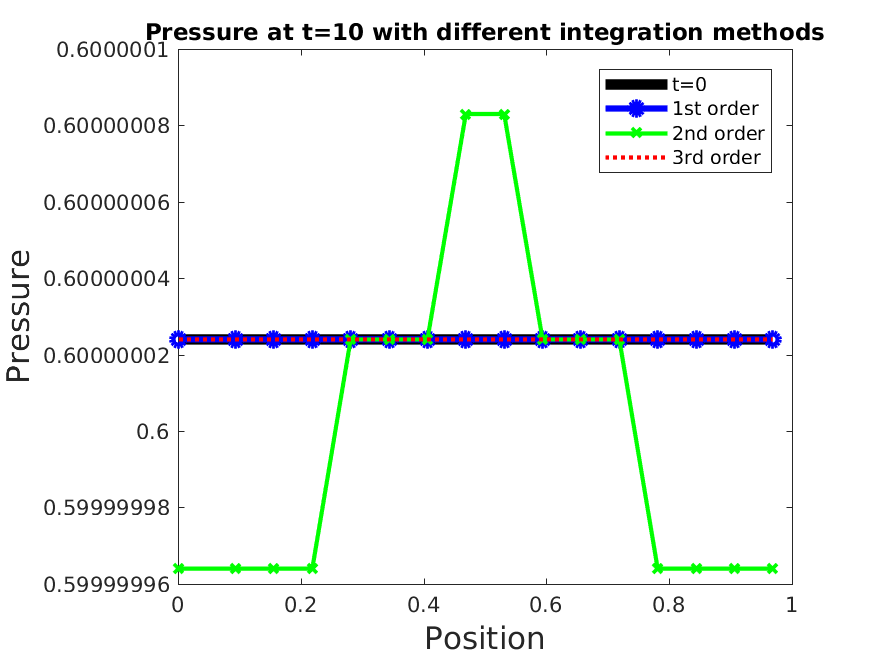
\includegraphics[width=.475\textwidth]{lw2prs.png}
	\end{tabular}
  \end{center}
  \caption{Results from linear waves tests, showing density (top), velocity (bottom left) and pressure (bottom right) computed using different integration methods and compared with an initial condition.}
  \label{fig:lw2}
\end{figure}
\clearpage

\subsection{Test 1: Sod's Shock Tube} 
The Sod's Shock tube test features examples of three different types of waves. A shock wave appears around $x=0.85$. A contact discontinuity appears around $x=0.68$. A rarefaction wave appears between about $x=0.3$ and $x=0.5$. 

First, the tests were run with values computed at different intervals; the method of integration is the same in each test. Between the two endpoints, 128, 256, 512, and 1024 points were computed for on each respective test. Figure~\ref{fig:dencellcomp_20} shows results of these tests:
\begin{figure}[h!]
  \begin{center}
    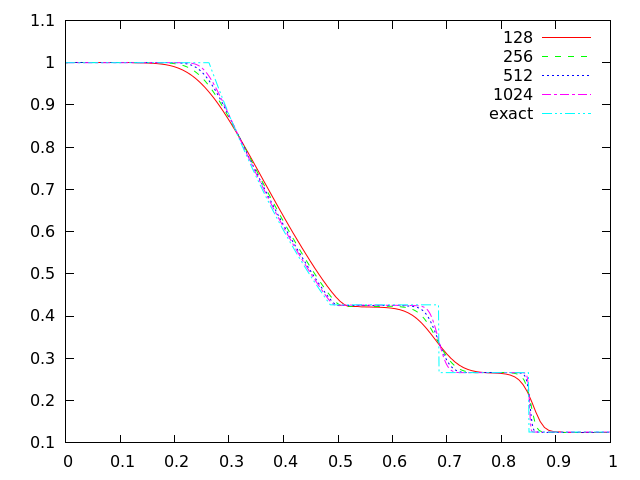
\includegraphics[width=.95\textwidth]{dencellcomp_20}
    \begin{tabular}{cc}
      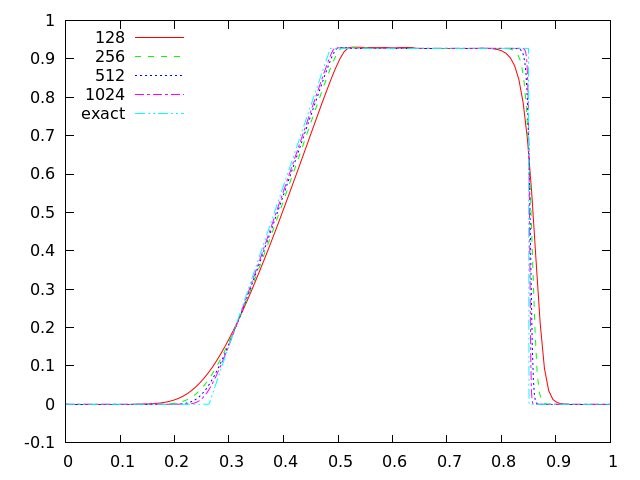
\includegraphics[width=.475\textwidth]{velcellcomp_20} &
      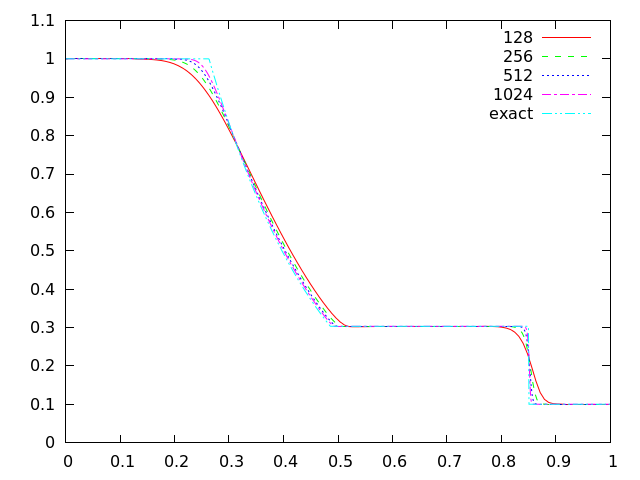
\includegraphics[width=.475\textwidth]{prscellcomp_20}
    \end{tabular}
  \end{center}
  \caption{Results showing the density (top), velocity (bottom left), and pressure (bottom right) for Sod's shock tube at $t=0.2$, computed with the first-order method using different number of elements: 128 (solid red), 256 (dashed green), 512 (dotted blue), and 1024 (dash-dot pink).  The exact solution, obtained with Toro's Riemann solver, is given by the dash-dotted cyan line.}
  \label{fig:dencellcomp_20}
\end{figure}

Next, several tests were run of different integration methods; the number of points was held constant at 128 each time. Higher numbers in the key correspond to higher-order, more exact methods of integration. 

\begin{figure}[h]
  \begin{center}
    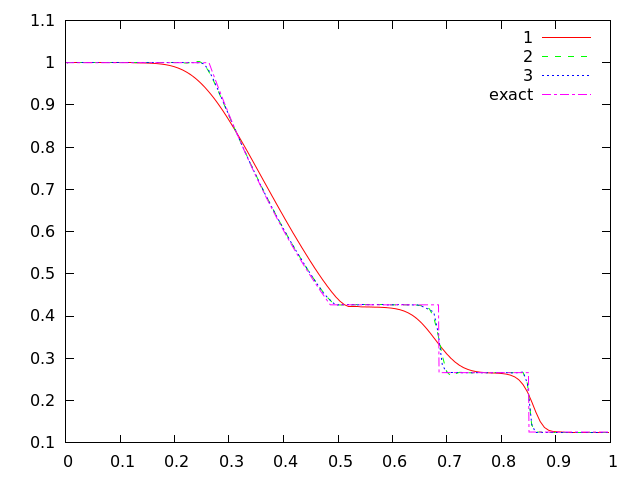
\includegraphics[width=.975\textwidth]{den128comp_20}
    \begin{tabular}{cc}
      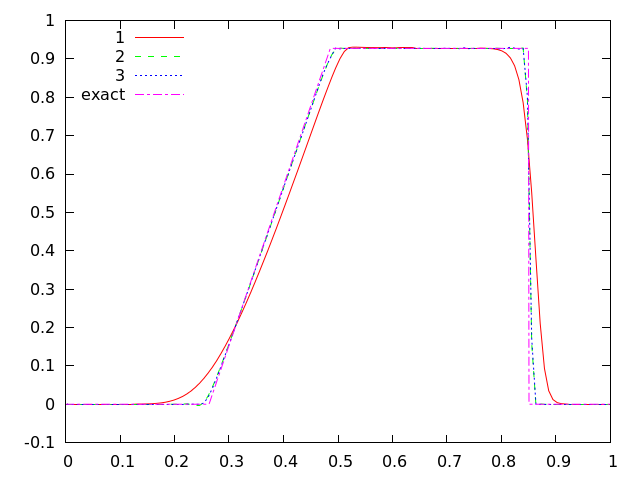
\includegraphics[width=.475\textwidth]{vel128comp_20} &
      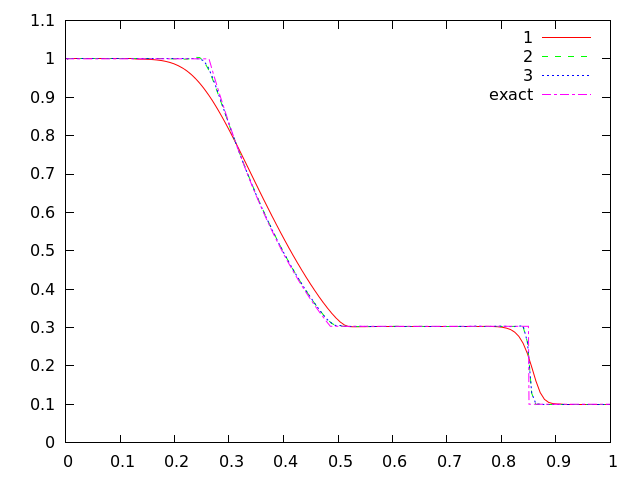
\includegraphics[width=.475\textwidth]{prs128comp_20}
    \end{tabular}
  \end{center}
  \caption{Results showing the density (top), velocity (bottom left), and pressure (bottom right) for Sod's shock tube at $t=0.2$, computed with 128 cells with methods of different orders: 1st (solid red), 2nd (dashed green) and 3rd (dotted blue). The exact solution, obtained with Toro's Riemann solver, is given by the dash-dotted pink line.}
  \label{fig:den128comp}
\end{figure}


These graphs show that the combination of both the lowest order integration method and 128 points yields significant error; however, improving either the method of integration or the number of points gives a solution much closer to the exact solution. 

\clearpage

\subsection{Test 2: Toro's Riemann Problem}

This test is the same as Sod's shock tube from the previous section, except that there is a non-zero velocity to the left of the initial discontinuity.  
As a result, a sonic point develops in the rarefaction wave.  
For subsequent tests, the number of cells was consistent within each test, and the integration method was varied as in the first test. 
The graphs for the second test show a result common throughout many of the different tests: The first order integration method is considerably far from the exact solution; the second and third order integration methods yield nearly identical results which are near, but not exactly equal to, the exact solution. 
\begin{figure}[h]
  \begin{center}
     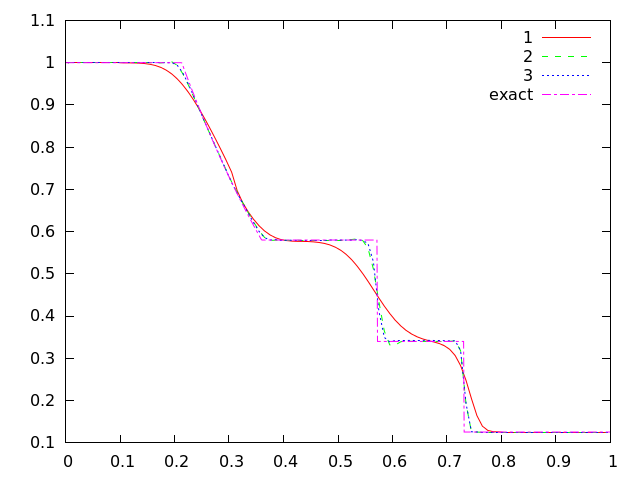
\includegraphics[width=.95\textwidth]{den_T2.png}
	 \begin{tabular}{cc}
      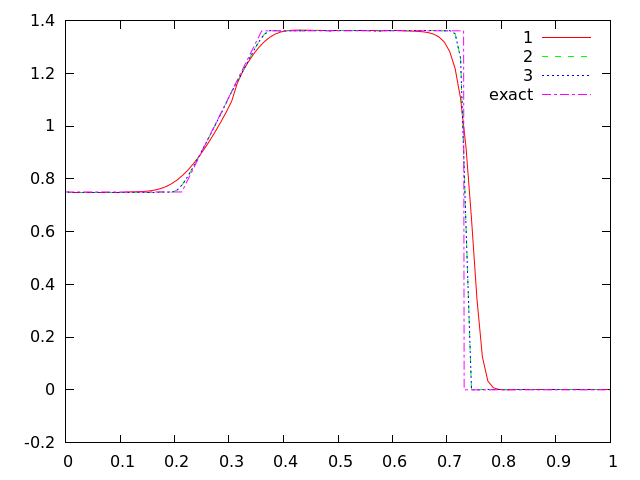
\includegraphics[width=.475\textwidth]{vel_T2.png} &
	  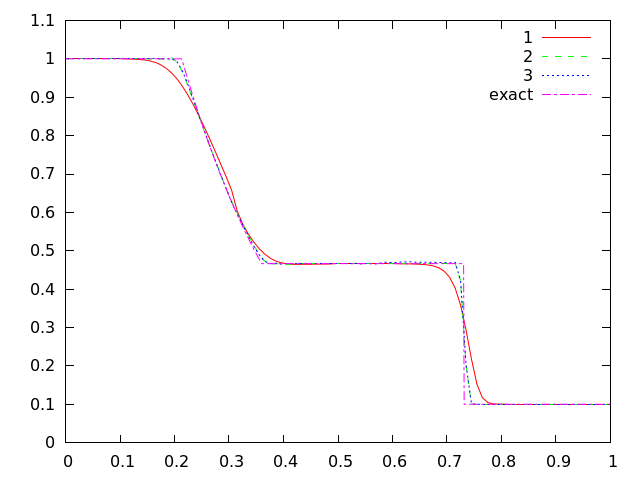
\includegraphics[width=.475\textwidth]{prs_T2.png}
	 \end{tabular}	
  \end{center}
  \caption{Results showing the density (top), velocity (bottom left), and pressure (bottom right) for test 2 at $t=0.2$, computed with 100 cells with methods of different orders: 1st (solid red), 2nd (dashed green) and 3rd (dotted blue). The exact solution, obtained with Toro's Riemann solver, is given by the dash-dotted pink line.}
  \label{fig:den_T2}
\end{figure}


\clearpage

\subsection{Test 3: Double Rarefaction}
This test features two rarefaction waves. They are moving in opposite directions, away from the initial discontinuity in the center. 

This test shows results similar to Toro's Riemann Problem. The deviation of experimental results from exact is especially noticeable in velocity. Near the initial point of discontinuity, the exact results appear completely horizontal. Method 1 almost completely ignores this horizontal part, while Methods 2 and 3 smooth it out considerably. 
\begin{figure}[h]
  \begin{center}
     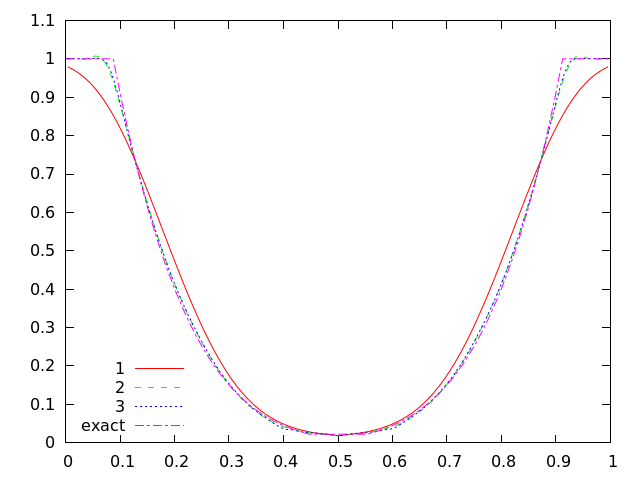
\includegraphics[width=.95\textwidth]{den_T3.png}	
	\begin{tabular}{cc}
      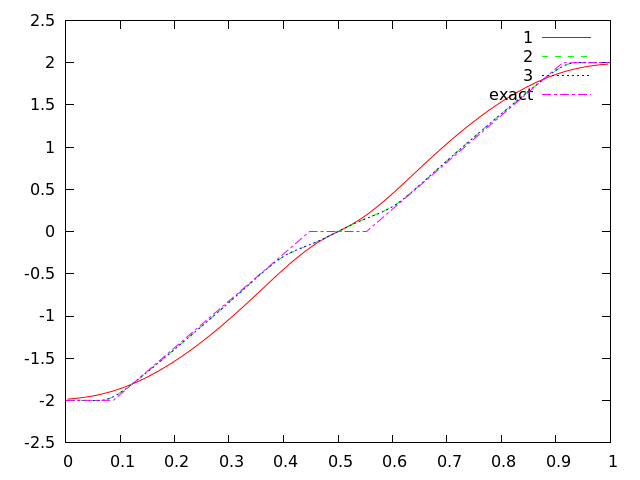
\includegraphics[width=.475\textwidth]{vel_T3.png} &
	  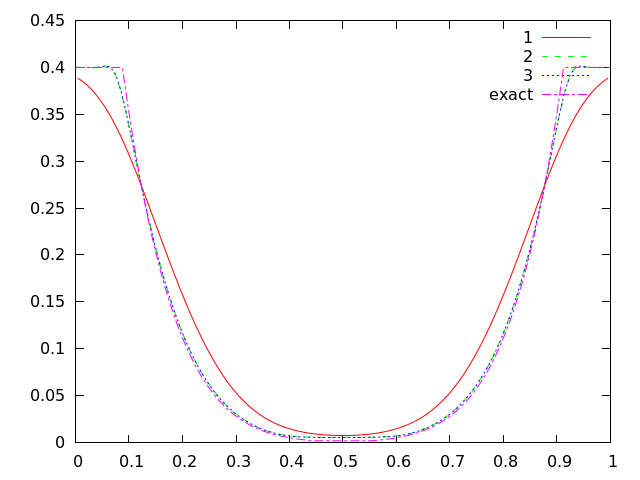
\includegraphics[width=.475\textwidth]{prs_T3.png}
	\end{tabular}
  \end{center}
  \caption{Results showing the density (top), velocity (bottom left), and pressure (bottom right) for the double rarefaction problem at $t=0.15$, computed with 100 cells with methods of different orders: 1st (solid red), 2nd (dashed green) and 3rd (dotted blue). The exact solution, obtained with Toro's Riemann solver, is given by the dash-dotted pink line.}
  \label{fig:den_T3}
\end{figure}


\clearpage

\subsection{Test 4: Noh}
The Noh problem features two shock waves. One is located near $x=0.28$, while the other is near $x=.82$.
This test obviously displays some difference from the exact solution in density. A depression appears in the center of the graph which is not part of the exact solution. This depression is most severe when method 1 is used, but it also appears with methods 2 and 3. Additionally, all three solutions show many small oscillations along horizontal lines. 

\begin{figure}[h]
  \begin{center}
     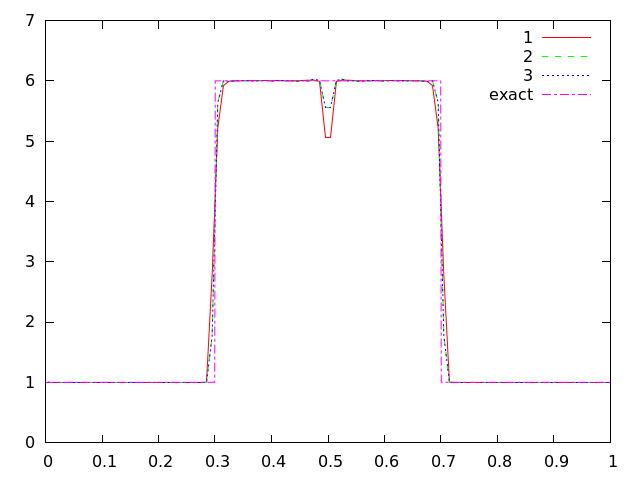
\includegraphics[width=.95\textwidth]{den_T4.png}	
	\begin{tabular}{cc}
      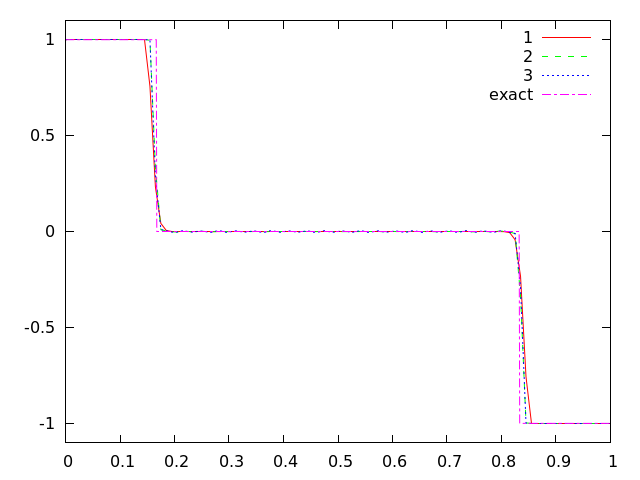
\includegraphics[width=.475\textwidth]{vel_T4.png} &
	  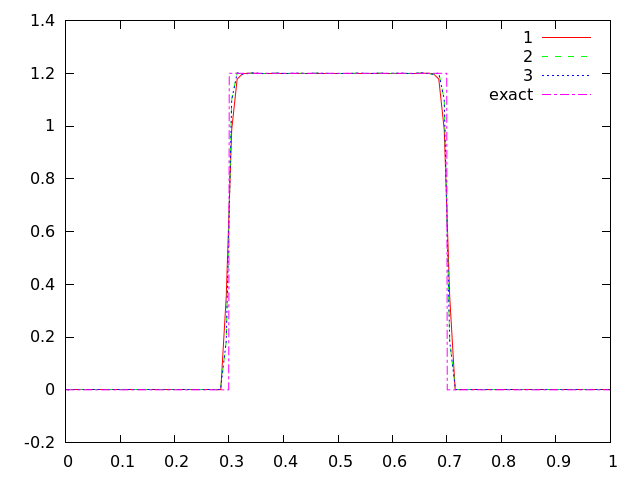
\includegraphics[width=.475\textwidth]{prs_T4.png}
	\end{tabular}
  \end{center}
  \caption{Results showing the density (top), velocity (bottom left), and pressure (bottom right) for the Noh problem at $t=1$, computed with 100 cells with methods of different orders: 1st (solid red), 2nd (dashed green) and 3rd (dotted blue). The exact solution, obtained with Toro's Riemann solver, is given by the dash-dotted pink line.}
  \label{fig:den_T4}
\end{figure}


\clearpage

\subsection{Test 5}
This test features three different types of waves. A shock wave appears around $x=0.85$. A contact discontinuity appears at $x=0.8$. A rarefaction wave appears between $x=0.1$ and $x=0.4$.

This test has interesting features in velocity. The first integration method underestimates the velocity at positions between about 0.2 and 0.5. The second and third order methods find a bump in density at around 0.4, which is not present in the exact solution.

\begin{figure}[h]
  \begin{center}
     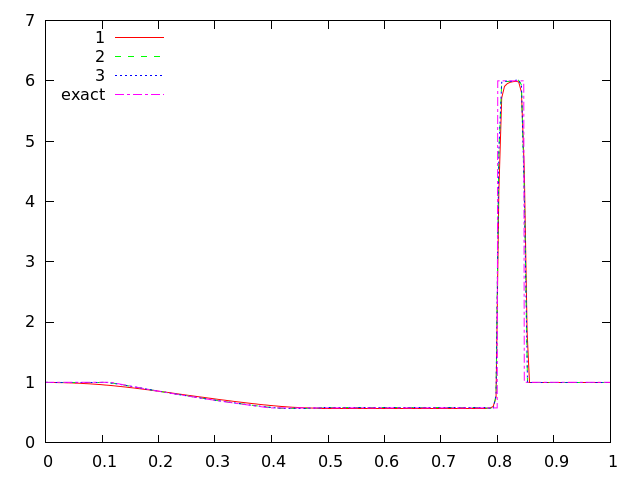
\includegraphics[width=.95\textwidth]{den_T5.png}
	\begin{tabular}{cc}
      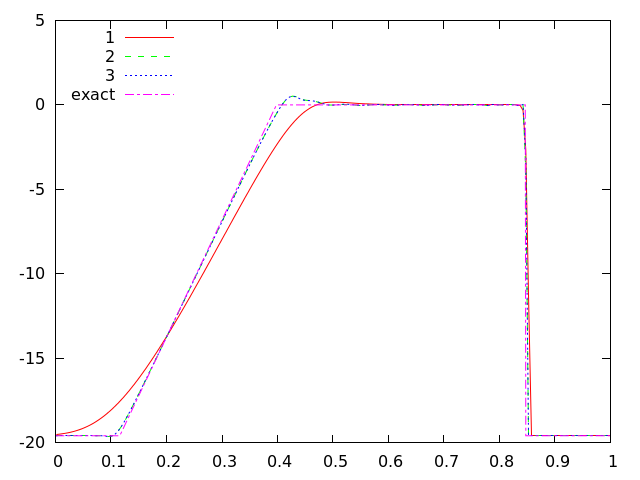
\includegraphics[width=.475\textwidth]{vel_T5.png} &
	  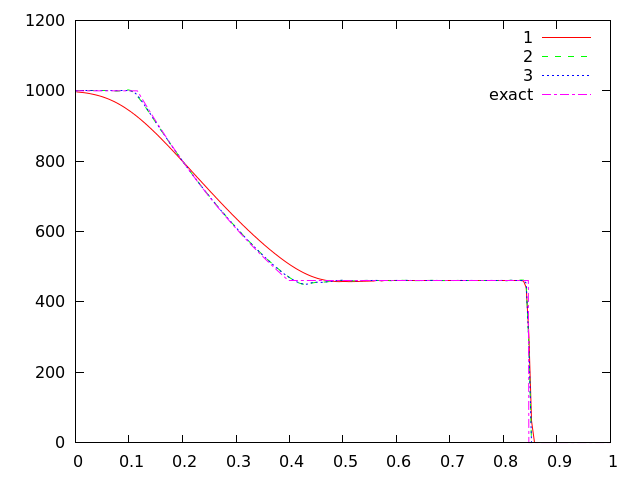
\includegraphics[width=.475\textwidth]{prs_T5.png}
	\end{tabular}	
  \end{center}
  \caption{Results showing the density (top), velocity (bottom left), and pressure (bottom right) for test 5 at $t=0.012$, computed with 200 cells with methods of different orders: 1st (solid red), 2nd (dashed green) and 3rd (dotted blue). The exact solution, obtained with Toro's Riemann solver, is given by the dash-dotted pink line.}
  \label{fig:den_T5}
\end{figure}


\subsection{Test 6}
This test features two shock waves, one around $x=0.85$ and the other around $x=0.42$. It also features a contact discontinutiy at $x=0.7$.
For this test's pressures and velocity, all three integration methods give values very close to exact. However, method 1 proves to be quite bad--worse than usual--at computing the density for this test. 

\begin{figure}[h]
  \begin{center}
     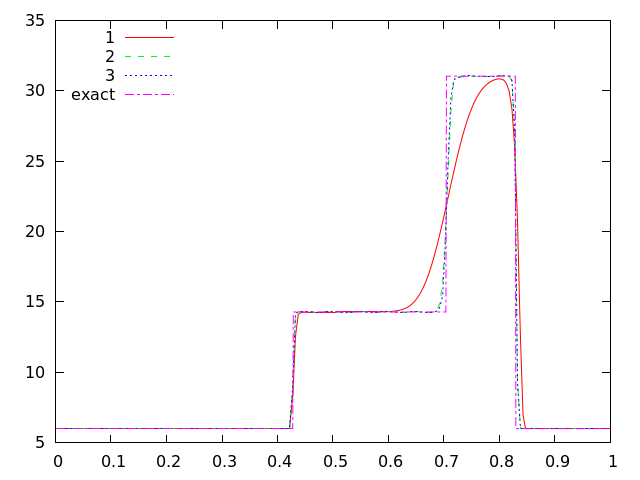
\includegraphics[width=.95\textwidth]{den_T6.png}	
	\begin{tabular}{cc}
      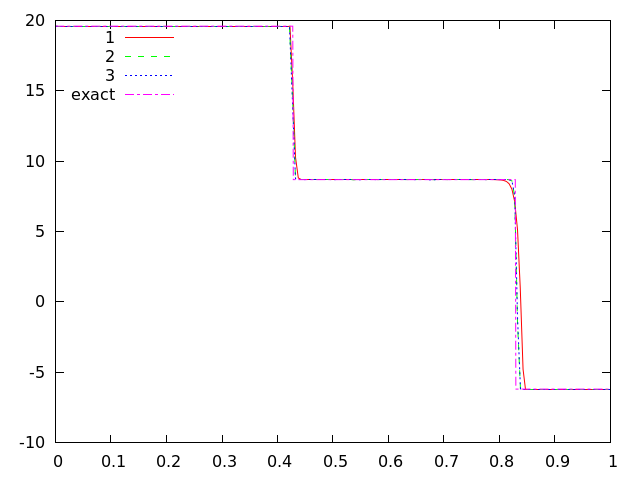
\includegraphics[width=.475\textwidth]{vel_T6.png} &
	  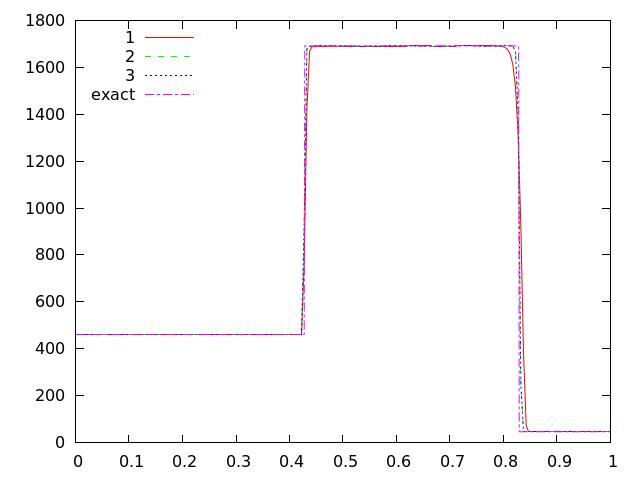
\includegraphics[width=.475\textwidth]{prs_T6.png}
	\end{tabular}
  \end{center}
  \caption{Results showing the density (top), velocity (bottom left), and pressure (bottom right) for test 6 at $t=0.035$, computed with 200 cells with methods of different orders: 1st (solid red), 2nd (dashed green) and 3rd (dotted blue). The exact solution, obtained with Toro's Riemann solver, is given by the dash-dotted pink line.}
  \label{fig:den_T6}
\end{figure}


\clearpage

\subsection{Test 7: Stationary Contact Discontinuity}
This test features a contact discontinuity at $x=0.5$. This test features an unusual situation--method 1 calculates the velocity exactly, while method 2 introduces more error and method 3 introduces the most. However, this graph only appears extreme because the intervals on its axis are so small. The numbers are always very close to zero, but very slight errors occur in some of the computations. 

\begin{figure}[h]
  \begin{center}
     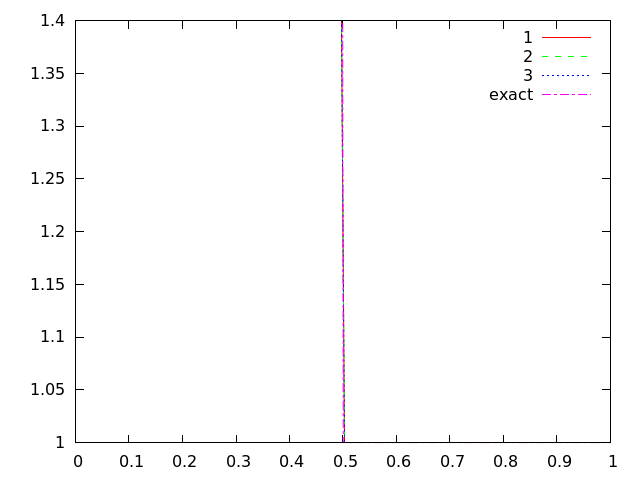
\includegraphics[width=.95\textwidth]{den_T7.png}	
	\begin{tabular}{cc}
      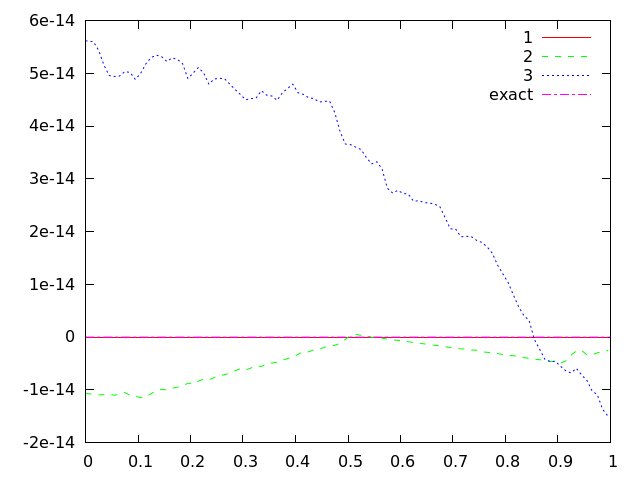
\includegraphics[width=.475\textwidth]{vel_T7.png} &
	  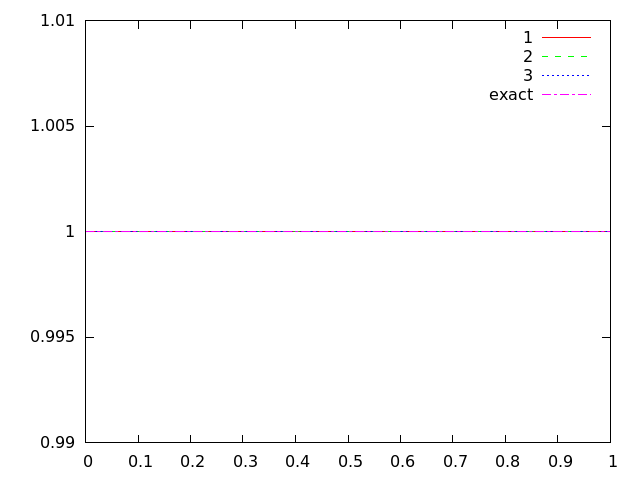
\includegraphics[width=.475\textwidth]{prs_T7.png}
	\end{tabular}
  \end{center}
  \caption{Results showing the density (top), velocity (bottom left), and pressure (bottom right) for the stationary contact discontinuity test at $t=2$, computed with 100 cells with methods of different orders: 1st (solid red), 2nd (dashed green) and 3rd (dotted blue). The exact solution, obtained with Toro's Riemann solver, is given by the dash-dotted pink line.}
  \label{fig:den_T7}
\end{figure}


\clearpage

\subsection{Test 8: Moving Contact Discontinuity}
This test features a contact discontinuity at $x=0.7$. In density, this test shows a small blip around $x=0.7$ that is unique to the second order method. Velocity and pressure are both constant throughout. 
\begin{figure}[h]
  \begin{center}
     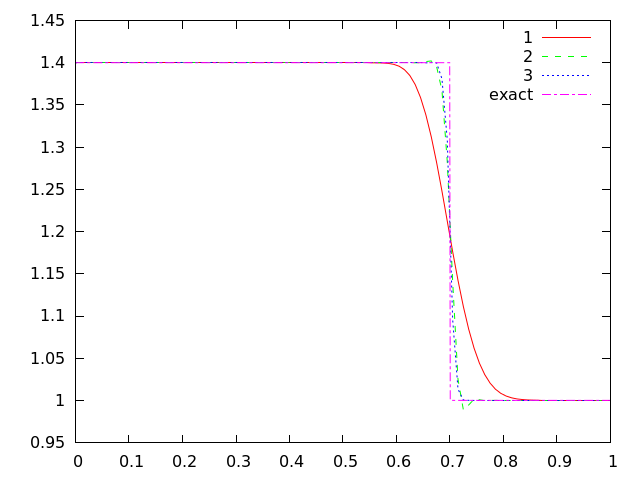
\includegraphics[width=.95\textwidth]{den_T8.png}
	\begin{tabular}{cc}
      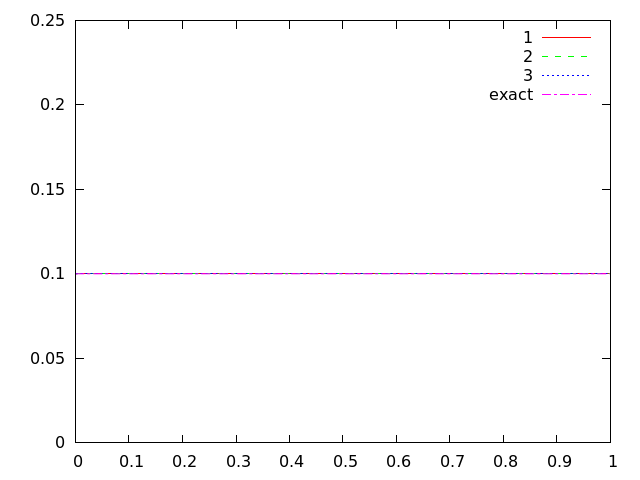
\includegraphics[width=.475\textwidth]{vel_T8.png} &
	  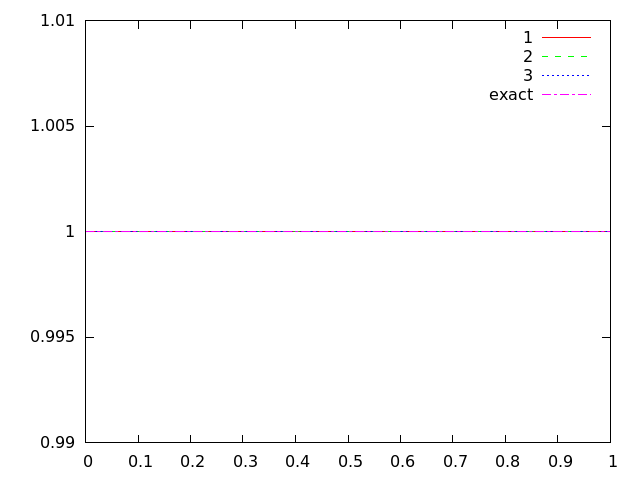
\includegraphics[width=.475\textwidth]{prs_T8.png}
	\end{tabular}
  \end{center}
  \caption{Results showing the density (top), velocity (bottom left), and pressure (bottom right) for the moving contact discontinuity test at $t=2$, computed with 100 cells with methods of different orders: 1st (solid red), 2nd (dashed green) and 3rd (dotted blue). The exact solution, obtained with Toro's Riemann solver, is given by the dash-dotted pink line.}
  \label{fig:den_T8}
\end{figure}


\clearpage

\subsection{Test 9: Peak}
The peak problem features a shock wave at $x=0.554$, as well as a contact discontinuity at $x=0.546$. A rarefaction wave is also present between about $x=0.16$ and $x=0.2$. When finding density, method 1 falls considerably short of the maximum. On the pressure graph, method 3 features both a jump above and a dip below the graph between positions 0.1 and 0.2. Velocity shows a similar (but considerably larger) dip, followed by jump, in the vertical section of the graph between 0.1 and 0.2. Method 1 also overestimates the maximum velocity and is above both exact and method 3 in the middle horizontal section. 

\begin{figure}[h]
  \begin{center}
	\begin{tabular}{cc}
      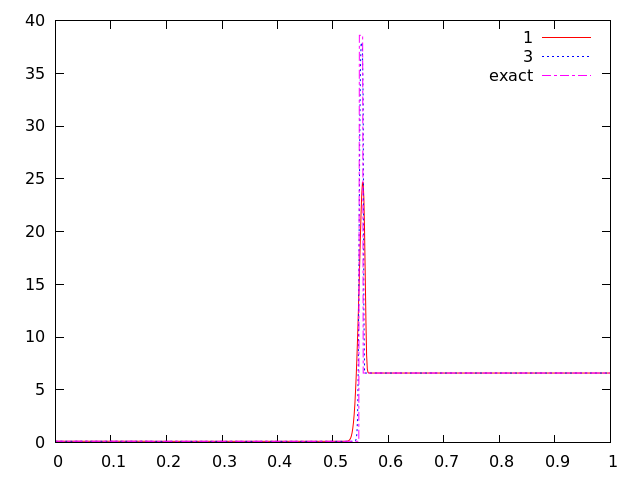
\includegraphics[width=.4\textwidth]{den_T9.png} &
	  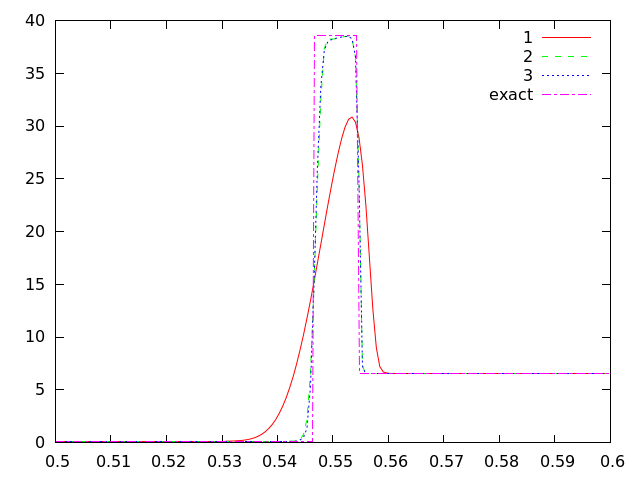
\includegraphics[width=.4\textwidth]{denT9zoom.png} \\
	  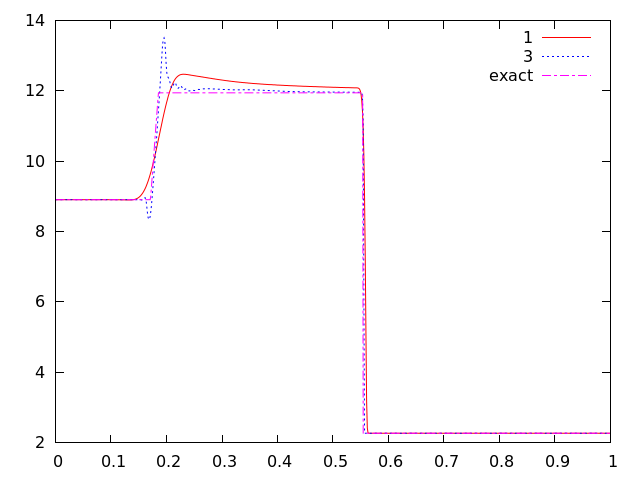
\includegraphics[width=.4\textwidth]{vel_T9.png} &	
      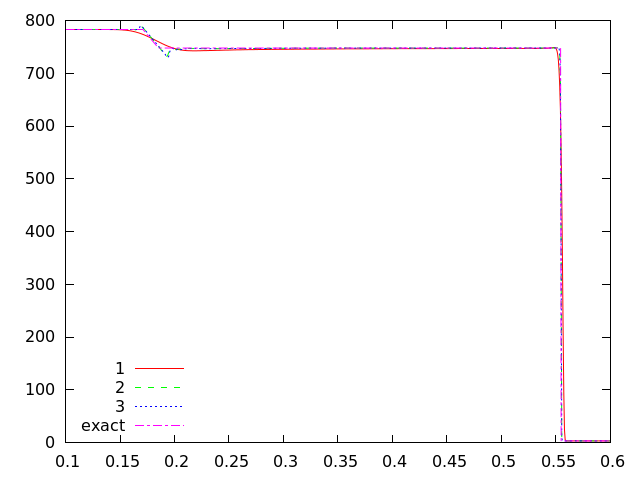
\includegraphics[width=.4\textwidth]{prs_T9.png}\\
	\end{tabular}	
  \end{center}
  \caption{Results for the peak problem at $t=0.0039$, computed with 800 cells with methods of different orders: 1st (solid red), 2nd (dashed green) and 3rd (dotted blue). The exact solution, obtained with Toro's Riemann solver, is given by the dash-dotted pink line. Density is shown in the top two panels at two different zoom levels. The bottom left panel shows velocity, and the bottom right panel shows pressure.}
\end{figure}


\clearpage

\subsection{Test 10: Start-up Errors}

In this problem, a shock wave is present at about $x=11$. Density, pressure, and velocity all show significant oscillations that follow the shock wave. These oscillations are not part of the exact solution, and appear to a different extend based on the integration method used. First order gives a few wide oscillations; higher order methods give more, taller, and thinner oscillations, with the third order giving the most. 
\begin{figure}[h]
  \begin{center}
	\begin{tabular}{cc}
      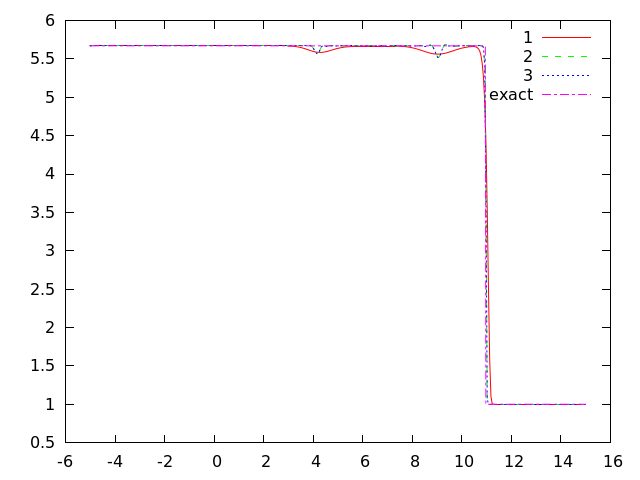
\includegraphics[width=.4\textwidth]{den_T10.png} &
	  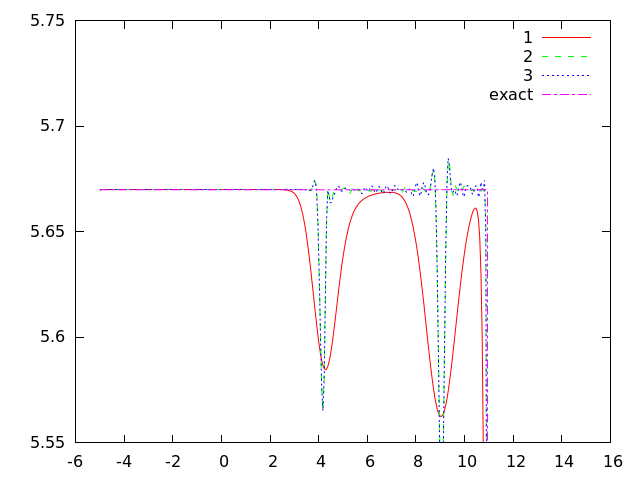
\includegraphics[width=.4\textwidth]{den10zoom.png} \\
	  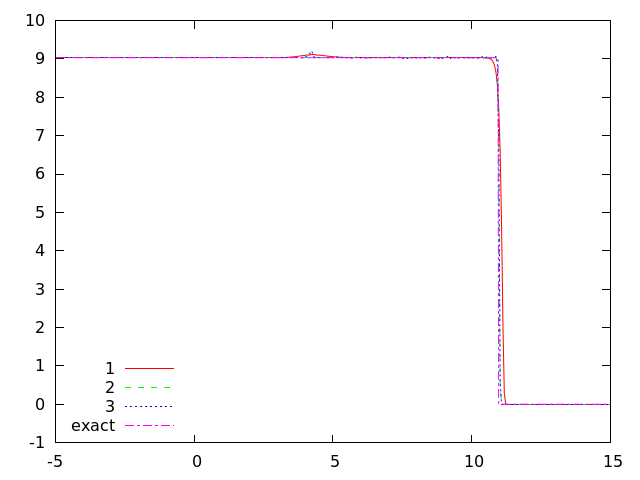
\includegraphics[width=.4\textwidth]{vel_T10.png} &	
	  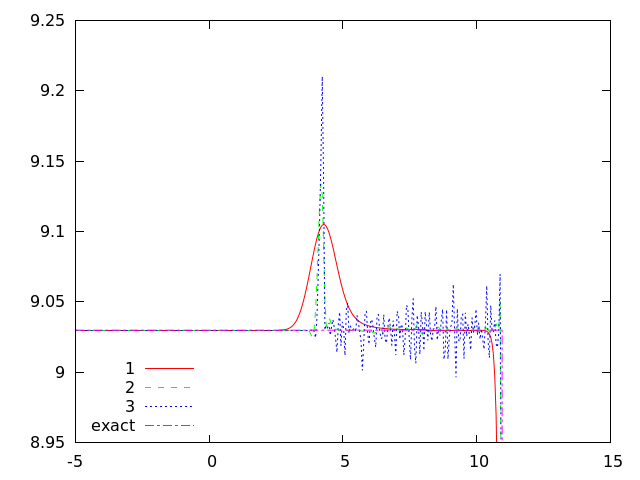
\includegraphics[width=.4\textwidth]{vel10zoom.png} \\
      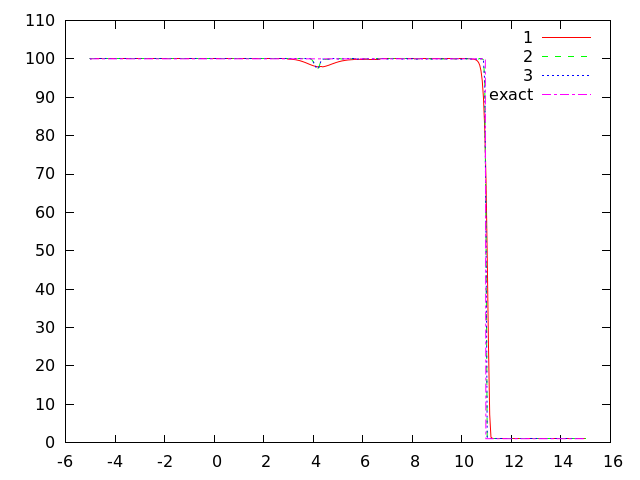
\includegraphics[width=.4\textwidth]{prs_T10.png} &	
      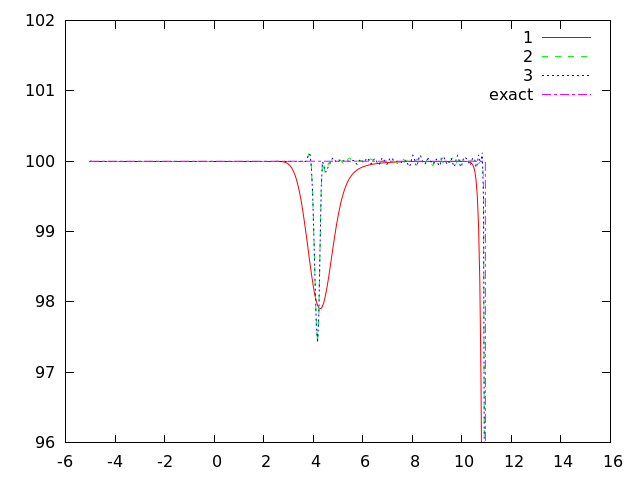
\includegraphics[width=.4\textwidth]{prs10zoom.png} \\
	\end{tabular}	
  \end{center}
  \caption{Results for test 10 at $t=1$, computed with 400 cells with methods of different orders: 1st (solid red), 2nd (dashed green) and 3rd (dotted blue). The exact solution, obtained with Toro's Riemann solver, is given by the dash-dotted pink line. Each pair of side-by-side panels shows the same results at different zoom levels. The top panels show density, the middle show velocity, and the bottom show pressure.}
\end{figure}



\clearpage

\subsection{Test 11: Slow-moving Shock}
In this problem, a shock wave is present at about $x=0.5$.This test, like the previous one, shows significant oscilltions following the shock wave, particularly with higher order methods. However, these oscillations in the second and third order results appear to be more periodic than those in the previous test. 
\begin{figure}[h]
  \begin{center}
	\begin{tabular}{cc}
      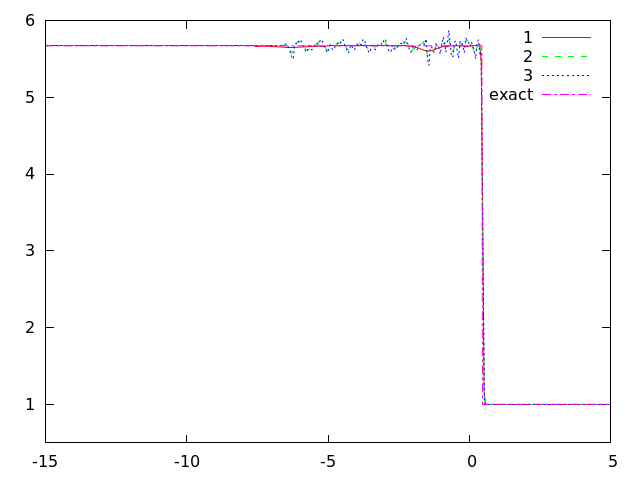
\includegraphics[width=.4\textwidth]{den_T11.png} &
	  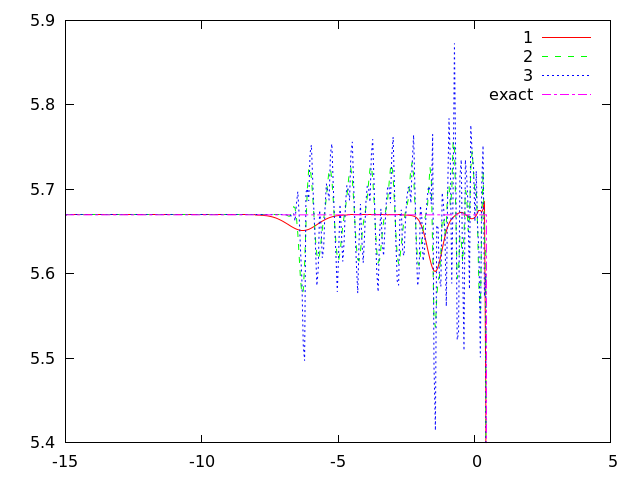
\includegraphics[width=.4\textwidth]{den11zoom.png} \\
	  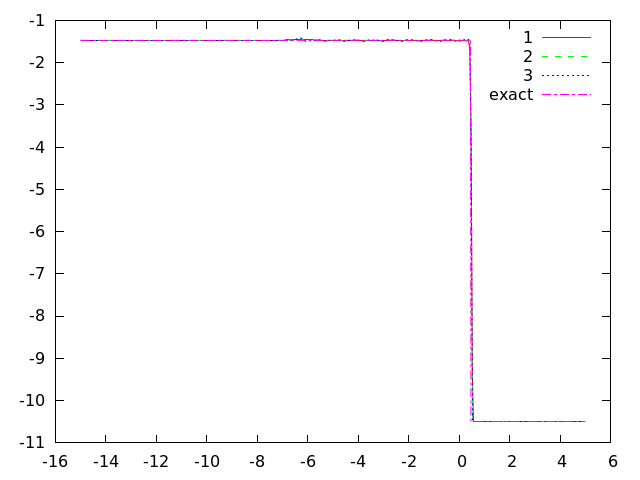
\includegraphics[width=.4\textwidth]{vel_T11.png} &	
	  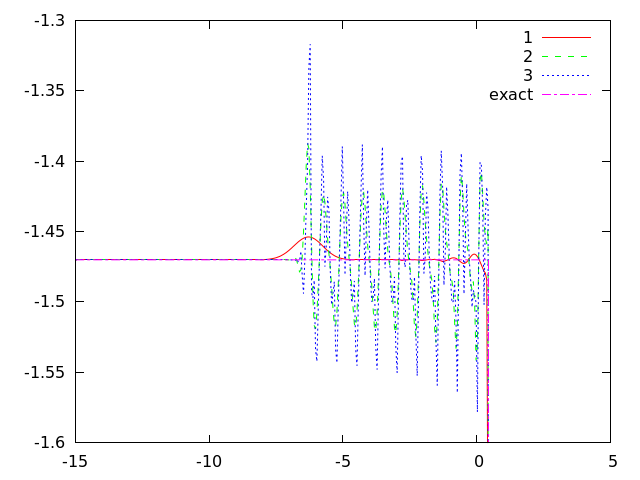
\includegraphics[width=.4\textwidth]{vel11zoom.png} \\
      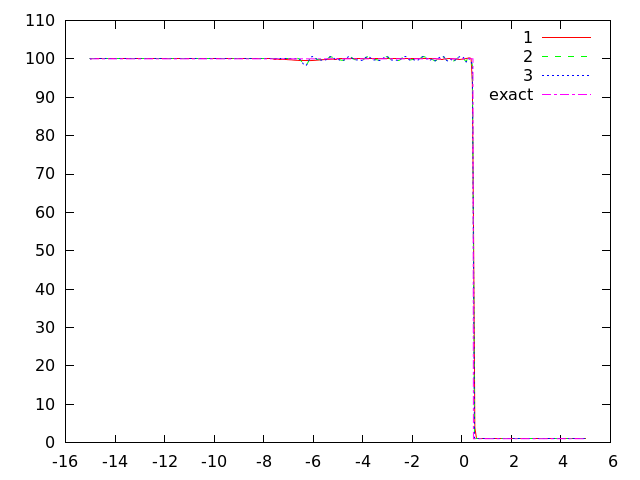
\includegraphics[width=.4\textwidth]{prs_T11.png} &	
      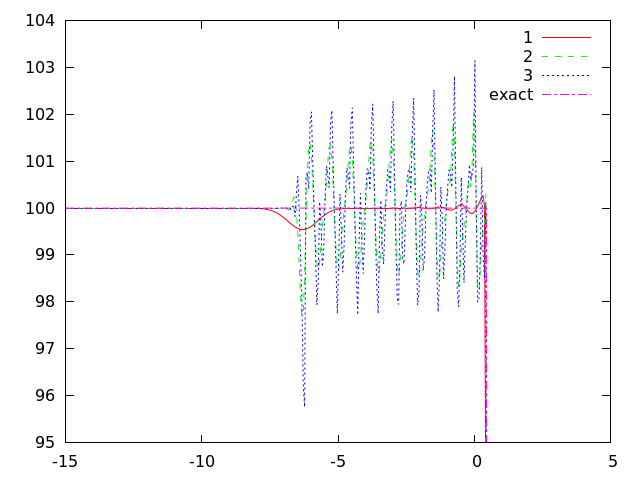
\includegraphics[width=.4\textwidth]{prs11zoom.png} \\
	\end{tabular}	
  \end{center}
  \caption{Results for test 11 at $t=1$, computed with 400 cells with methods of different orders: 1st (solid red), 2nd (dashed green) and 3rd (dotted blue). The exact solution, obtained with Toro's Riemann solver, is given by the dash-dotted pink line. Each pair of side-by-side panels shows the same results at different zoom levels. The top panels show density, the middle show velocity, and the bottom show pressure.}
\end{figure}

Subsequent runs of this test varied the values of $\beta_{\mbox{\tiny TVB}}$ and $\beta_{\mbox{\tiny TVD}}$, while maintaining the third order method. Lower values of $\beta_{\mbox{\tiny TVB}}$ give more accurate results, with fewer, smaller oscillations appearing. Variations in $\beta_{\mbox{\tiny TVD}}$ have some effect, but not a great one. A few of the oscillations appear larger with $\beta_{\mbox{\tiny TVD}}$ set to 1.0, but the difference is not especially large.

\begin{figure}[h]
  \begin{center}
     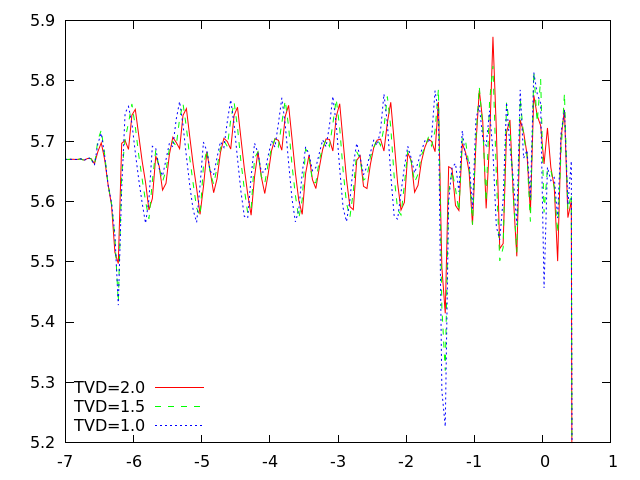
\includegraphics[width=.95\textwidth]{11_300zoom.png}	
	\begin{tabular}{cc}
     \includegraphics[width=.475\textwidth]{11_1zoom.png}
     \includegraphics[width=.475\textwidth]{11_2zoom.png}	
    \end{tabular}
  \end{center}
  \caption{Zoomed results for test 11 at $t=1$, computed with 400 cells and the third order method. The top panel shows results when $\beta_{\mbox{\tiny TVB}}$ is set to 300, with varying values of $\beta_{\mbox{\tiny TVD}}$: 1.0 (dotted blue), 1.5 (dashed green) and 2.0 (solid red). The bottom two panels show results when $\beta_{\mbox{\tiny TVD}}$ is held constant, with varying values of $\beta_{\mbox{\tiny TVB}}$: 0 (solid red), 10 (dashed green), 50 (dotted blue), and 300 (dash-dotted pink). $\beta_{\mbox{\tiny TVD}}$ is set to 1.0 in the right panel and 2.0 in the left panel.}
\end{figure}
\clearpage

\subsection{Test 12: Interacting Blast Waves}
This test was run for all three integration methods with both 400 cells and 2000 cells. Since it has no exact solution, the 2000 cell, third order test is compared to all three 400 cell tests and labeled as ``exact.''

\begin{figure}[h]
  \begin{center}
     \includegraphics[width=.95\textwidth]{den_T12_2000.png}
	\begin{tabular}{cc}
     \includegraphics[width=.475\textwidth]{vel_T12_2000.png}
     \includegraphics[width=.475\textwidth]{prs_T12_2000.png}	
    \end{tabular}	
  \end{center}
  \caption{Results showing the density (top), velocity (bottom left), and pressure (bottom right) for the Woodward-Collela blast wave problem at $t=0.038$, computed with 2000 cells with methods of different orders: 1st (solid red), 2nd (dashed green) and 3rd (dotted blue).}
  \label{fig:den_T12_2000}
\end{figure}


\begin{figure}[h]
  \begin{center}
     \includegraphics[width=.95\textwidth]{den_T12_400.png}	
	\begin{tabular}{cc}
     \includegraphics[width=.475\textwidth]{vel_T12_400.png}
     \includegraphics[width=.475\textwidth]{prs_T12_400.png}	
    \end{tabular}
  \end{center}
  \caption{Results for the density (top), velocity (bottom left), and pressure (bottom right) from the same experiments as shown in Figure~\ref{fig:den_T12_2000}~computed with 400 cells. The solution labelled ``exact' and given by the dash-dotted pink line is the results of the problem when computed using the third-order integration method with 2000 cells.}
  \label{fig:den_T12_400}
\end{figure}


\clearpage

\subsection{Test 13: Shock-Entropy Wave Interaction}

This test was first run with 1000 cells to see the solution with high resolution. Subsequent tests all had 200 cells, with various values of the beta parameter. Again, the 3rd order, 1000 cell solution is called ``exact.''

This test features many oscillations that are part of the real solution. In the higher-resolution runs, at least the second order integration method was needed to show these oscillations. In the lower-resolutions, when beta was set to 10, 2nd and 3rd order yielded similar results, both greatly smoothing out the oscillations. When beta was 50, 3rd order outperformed 2nd, but both were still insufficient to model the oscillations. Beta set to 300 yielded the most accurate results, and the 3rd order results were especially accurate. 

\begin{figure}[h]
  \begin{center}
     \includegraphics[width=.95\textwidth]{1000.png}	
  \end{center}
  \caption{Results showing the density for the Shock Entropy Wave problem at $t=1.8$, computed with 1000 cells with methods of different orders: 1st (solid red), 2nd (dashed green) and 3rd (dotted blue).}
  \label{fig:shock}
\end{figure}

\begin{figure}
  \begin{center}
	\begin{tabular}{cc}
      \includegraphics[width=.475\textwidth]{10.png} &
	  \includegraphics[width=.475\textwidth]{10zoom.png}
	\end{tabular}
  \end{center}
  \caption{Results from the same experiments as shown in Figure~\ref{fig:shock}~at two different zoom levels, computed with 200 cells and beta set to 10. The solution labelled ``exact' and given by the dotted blue line is the results of the problem when computed using the third-order integration method with 2000 cells.}
\end{figure}

\begin{figure}
  \begin{center}
	\begin{tabular}{cc}
      \includegraphics[width=.475\textwidth]{50.png} &
	  \includegraphics[width=.475\textwidth]{50zoom.png}
	\end{tabular}
  \end{center}
  \caption{Results from the same experiments as shown in Figure~\ref{fig:shock}~at two different zoom levels, computed with 200 cells and beta set to 50.}
\end{figure}

\begin{figure}
  \begin{center}
	\begin{tabular}{cc}
      \includegraphics[width=.475\textwidth]{300.png} &
	  \includegraphics[width=.475\textwidth]{300zoom.png}
	\end{tabular}
  \end{center}
  \caption{Results from the same experiments as shown in Figure~\ref{fig:shock}~at two different zoom levels, computed with 200 cells and beta set to 300.}
\end{figure}


\section{Conclusion}
The thornado code was benchmarked using a large suite of Riemann problem tests. In all of these tests, the code was able to capture the structure of the problem well. In general, using a second order integration method instead of a first order integration method greatly increased the accuracy of the solution. For tests in which constant states were separated by a discontinuity, changing from second to third order brought little improvement. However, the difference between these methods was significant in the Shock Entropy Waves test—third order showed a much greater ability to follow oscillations when beta was set to 300. With smaller values of beta, the ability of the third order method to capture these oscillations was diminished, as was the difference between the second and third order methods. The tunable parameter beta is problematic because its optimal value is dependent on the features of the problem; it is impossible to choose a correct value of beta that can be used generally, in all situations. 

\bibliographystyle{apj}
\bibliography{references.bib}

\end{document}
